\documentclass[10pt]{article}
\usepackage[a4paper,margin=2.2cm]{geometry}
\usepackage{booktabs,graphicx,hyperref,xcolor,amsmath}
\hypersetup{colorlinks=true,linkcolor=blue!50!black,urlcolor=blue!50!black}
\newcommand{\repo}{https://github.com/charleneleong-ai/nebius-physical-ai}

\title{Preflight: making an SO-101 policy generalise to new scenes, objects and tasks\\
\large Experiments, funnels and verdicts (simulation only)}
\author{Preflight, Nebius $\times$ NVIDIA Physical AI hackathon}
\date{11 October 2026}

\begin{document}
\maketitle

\begin{abstract}
We fine-tune GR00T~N1.7 for pick-and-place on a MuJoCo twin of the SO-101 arm and try seven ways to make it
generalise. Every candidate is scored on the same six paired suites (96 rehearsals each) against the v5 baseline, with
scene-by-scene McNemar tests and a promotion gate. DAgger with upweighted expert recoveries is the one lever that passes the gate, twice: round~2 (pooled $+26$ of 576 over v5) and round~3 ($+19$ more, now served). A fairly trained FLUX~3~Action LoRA
loses on every suite despite predicting the right actions open-loop. A third DAgger round is the first candidate to move
new objects (61 vs 50 of 96, $p=0.043$), though its pooled gain over round~2 is within noise. All results are in simulation; the physical arm has not been delivered.
\end{abstract}

\section{Setup}
\textbf{Policy.} \texttt{hqfang/groot-so100\_101} (GR00T~N1.7, pretrained on 1,209 SO-100/101 datasets), fine-tuned with
LeRobot~0.6.1. \textbf{v5} adds 800 scripted twin demos (12k steps, batch 8, lr $2.5\times10^{-5}$) and is the
baseline for every comparison.

\textbf{Benchmark.} Six suites, each 12 scenes $\times$ 8 perturbed rehearsals $=96$, seed 42:
\texttt{held\_out\_objects} (objects never in training), \texttt{seen\_vocabulary}, \texttt{clean\_many},
\texttt{clean\_top\_down\_many}, \texttt{real\_1\_pomade\_tin\_many}, \texttt{in\_path\_pomade\_tin\_many}. Re-running one
checkpoint moves a suite by up to $\pm9$, so differences are judged only by paired McNemar tests on the scenes where two
checkpoints disagree. A candidate is \emph{promoted} only with a pooled paired gain and no suite significantly worse; the
gate was fixed before any round was scored. External check: so101-benchmark \texttt{stack\_blue\_on\_red}, 50 episodes.

\textbf{Failure labels.} Each failed rehearsal is labelled by \texttt{FailureWatch}: \emph{no\_contact} (pick block never
moved), \emph{pushed}, \emph{dropped}, \emph{fell\_off}, \emph{holding} (still lifted at timeout), \emph{knocked\_place}.

\section{Experiments}

\subsection{DAgger with upweighted recoveries (the one that works)}
Each round rolls the current policy out on 200 fresh training scenes $\times$ 4 variants, snapshots every failure
(simulator state plus scene), keeps the most uncertain within a recording budget balanced across failure types, and lets
the scripted expert record a recovery from each kept state. Table~\ref{tab:funnel} gives the funnel with every
denominator; failed recoveries (the expert could not stack from the state) are counted, not dropped.

\begin{table}[h]\centering\small
\begin{tabular}{lrrrrr}\toprule
Round (policy) & Rollouts & Succeeded & Failures kept & Recovered & Recoveries in training\\\midrule
1 (v5) & 800 & 456 (57\%) & 207 of 330 recoverable & 85 (41\%) & 85 of 2,485 (3.5\%)\\
2 (v5) & 800 & 494 (62\%) & 189 of 296 recoverable & 72 (38\%) & 157 $\times8$ of 3,656 ($\approx34\%$)\\
3 (round 2) & 800 & 574 (72\%) & 146 of 197 recoverable & 59 (40\%) & 216 $\times8$ of 4,128\\
4 (round 3, RL expert) & 800 & 614 (77\%) & 120 of 165 recoverable & 88 (73\%) & 304 $\times8$ of 4,832\\
5 (round 3, RL $\times2$) & 800 & 610 (76\%) & 113 of 160 recoverable & 72 (64\%) & 216 $\times8$ + 160 $\times2$ of 4,448\\\bottomrule
\end{tabular}
\caption{DAgger funnels. ``Recoverable'' excludes \emph{holding}, which the open-loop expert cannot recover from a lifted
state. Round 3 harvests with round 2; round 4 with the promoted round-3 policy, and its recoveries are recorded by the residual RL expert.}\label{tab:funnel}
\end{table}

\begin{table}[h]\centering\small
\begin{tabular}{lrrrl}\toprule
Suite (of 96) & v5 & Round 1 & Round 2 & Round 2 vs v5\\\midrule
held\_out\_objects & 52 & 47 & 50 & $+12/-14$, $p=0.85$\\
seen\_vocabulary & 75 & 76 & 76 & $+8/-7$, $p=1.0$\\
clean\_many & 81 & 82 & 86 & $+7/-2$, $p=0.18$\\
clean\_top\_down\_many & 83 & 77 & 85 & $+6/-4$, $p=0.75$\\
real\_1\_pomade\_tin\_many & 74 & 78 & \textbf{86} & $\mathbf{+14/-2}$, $\mathbf{p=0.004}$\\
in\_path\_pomade\_tin\_many & 73 & 76 & 81 & $+13/-5$, $p=0.10$\\\midrule
pooled (of 576) & 438 & 436 & \textbf{464} & $+26$: \textbf{promoted}\\\midrule
Round 3 (vs round 2) & \multicolumn{3}{r}{481; held\_out 61 vs 50, $+18/-7$, $p=0.043$} & $+17$: kept\\
Round 3 retrained & \multicolumn{3}{r}{\textbf{483}; held\_out 57 vs 50, $p=0.30$} & $+19$: \textbf{promoted}\\
Round 4 (vs round 3) & \multicolumn{3}{r}{471; held\_out 49 vs 57, $p=0.17$} & $-12$: kept\\
Round 5 (vs round 3) & \multicolumn{3}{r}{455; held\_out 41 vs 57, $p=0.004$} & $-28$: discarded\\\bottomrule
\end{tabular}
\caption{Paired results. Round 1 (recoveries 3.5\% of training) was kept, not promoted. Round 2 upweighted them to about a
third and was promoted. Round-2 failures fell from 138 to 112 (\emph{no\_contact} $57\to33$) while \emph{dropped} and
\emph{holding} did not fall.}\label{tab:dagger}
\end{table}

\subsection{FLUX 3 Action, trained fairly}
A LoRA (rank 32) on \texttt{black-forest-labs/flux-3-action-so101}, trained on exactly v5's 800 demos (bridged into
FLUX's joint units by a per-joint quantile map) for exactly v5's volume (96k samples in 12k updates of 8), never
initialised from v5. It scores 50 of 576 against v5's 438, worse on every suite ($p<0.001$ each), and 0 of 7 on
so101-benchmark (stopped early: all timeouts). 358 of its 526 failures are \emph{no\_contact}. Executing 16 actions per
chunk instead of 32 does not help (held\_out 4 vs 3, clean\_many 2 vs 9, $p=0.039$ worse).

To separate the model from the data bridge we score its predicted chunk open-loop on 60 held-out demo frames, each fed
the 7 frames before it (FLUX conditions on 8). Table~\ref{tab:openloop} and Figure~\ref{fig:openloop}: the LoRA predicts
the demo's actions three times better than holding the pose at 32 steps ahead; zero-shot FLUX is no better than standing
still. The bridge sits inside this loop both ways. The closed-loop failure is therefore execution, not the mapping.

\begin{table}[h]\centering\small
\begin{tabular}{rrrr}\toprule
Steps ahead & Fair LoRA & Zero-shot FLUX & Hold pose\\\midrule
1 & 0.23 & 0.37 & 0.53\\ 8 & 1.08 & 2.26 & 2.47\\ 16 & 1.75 & 4.34 & 4.66\\ 32 & \textbf{2.71} & 8.19 & 8.24\\\bottomrule
\end{tabular}
\caption{Open-loop mean $|$action error$|$ (LeRobot joint units) on held-out demo frames.}\label{tab:openloop}
\end{table}

\begin{figure}[h]\centering
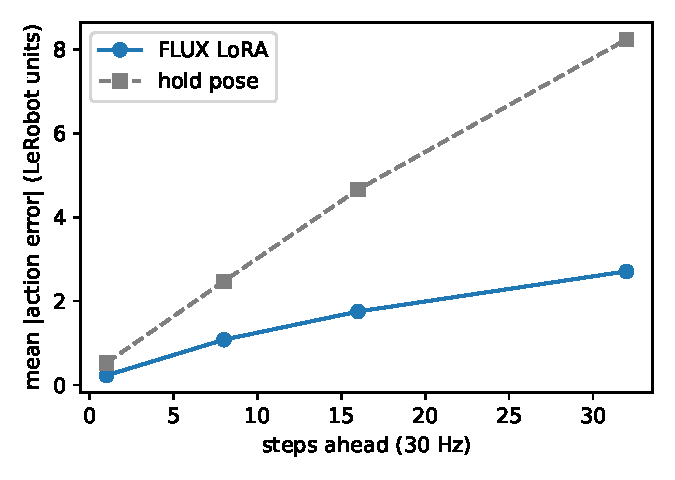
\includegraphics[width=0.48\linewidth]{figures/openloop_horizons_flux3-lora-v4c.pdf}\hfill
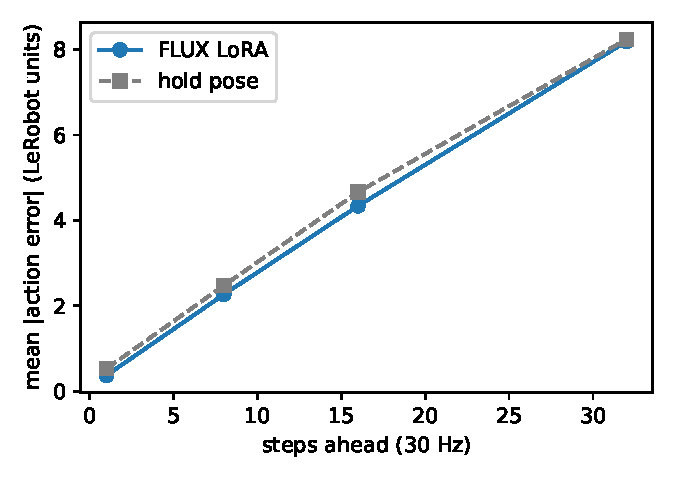
\includegraphics[width=0.48\linewidth]{figures/openloop_horizons_flux3-zeroshot.pdf}
\caption{Open-loop error against horizon: fair LoRA (left) and zero-shot FLUX (right), each beside holding the pose.}
\label{fig:openloop}
\end{figure}

\subsection{Other experiments}
\begin{itemize}\itemsep0pt
\item \textbf{Failure labels} (576 v5 rehearsals): no\_contact 41\%, pushed 25\%, dropped 17\% of failures.
\item \textbf{Targeted demos (v6)}: recoveries after staged mistakes plus lookalike decoys; within noise of v5 on every
suite.
\item \textbf{External benchmark gap}: v5 scores 0/50 on so101-benchmark; the joint mapping and front camera match, the
wrist-camera mount and table texture do not.
\item \textbf{Visual domain randomisation (v7)}: the Seeed wrist mount alone drops v5 from 81 to 15 on clean\_many's scenes;
v7 lifts that to 53 but regresses clean\_many itself to 58, and scores 1/50 externally. Not promoted.
\item \textbf{Real-data co-training (v9)}: 400 ArmnetBench SO-101 teleop demos of new objects at 23\% of samples score 373 vs 438;
held\_out\_objects 48 vs 52 ($p=0.59$), worse on clean\_many, clean\_top\_down\_many and real\_1\_pomade\_tin ($p\le0.043$), 0/50 externally.
Through the twin's kinematics 99.7\% of the teleop episodes put the gripper under the table; fitted joint offsets
($-6.0, -6.0, -5.1$ on the height-setting joints) cut that to 4.2\%. \textbf{v11}, round~3 fine-tuned with the 87 calibrated
block-stacking episodes at 9\%, scores 472 vs 483 with every suite within noise: calibrated real data no longer costs the twin.
\item \textbf{Best-of-8 consensus} (medoid of 8 sampled chunks, round 2): held\_out\_objects 55 vs 50 ($p=0.41$),
clean\_many 87 vs 86; within noise at $8\times$ inference.
\item \textbf{DiVeR verifier} (best-of-8 on round 3, after arXiv 2610.04933): an MLP on pooled backbone features, joints and
the chunk, trained on 300 round-3 rollouts (226 succeeded) with disagreement-weighted BCE, ranks held-out steps at AUC 0.79;
picking with it scores held\_out\_objects 54 vs 57 ($p=0.66$) and clean\_many 85 vs 88 ($p=0.51$).
\item \textbf{RL expert} (to replace the scripted expert): plain PPO on privileged state reached 1\% held-out recovery
by 4.4M steps and was stopped; the reward paid hovering more than stacking. A residual PPO policy on the scripted
expert, with potential-based shaping, recovers 74.0\% of held-out failure snapshots against the expert's 45.9\%.
\end{itemize}

\section{What is not established}
\begin{itemize}\itemsep0pt
\item \textbf{Nothing has run on the physical arm.} Every number is from the MuJoCo twin.
\item \textbf{The new-object gain is suggestive, not established.} Round 3's held\_out\_objects was 61 then 57 against round 2's
50 over two training runs; only the first is significant on its own ($p=0.043$, uncorrected).
\item \textbf{Round 2's gain is mostly one suite.} Only real\_1\_pomade\_tin is significant on its own; the other five are
better but within noise. The pooled gain passed a gate fixed in advance.
\item \textbf{Which half of the FLUX fix matters is open.} Retrained with current-frame conditioning and absolute joint targets
(a quarter of the budget), FLUX scores 21 vs 3 on held\_out\_objects ($p<0.001$), confirming the mechanism; the two changes
were made together, and it remains far below round~3.
\item \textbf{so101-benchmark remains 0--1 of 50} for every policy; the external gap is open.
\item \textbf{Single seed} for every benchmark (seed 42); no checkpoint was trained twice.
\end{itemize}

\section{Next}
Round~3 retrained and promoted (483); RL-expert recoveries in rounds~4 and~5 ($\times8$, $\times2$) scored 471 and 455 and are dropped.
Best-of-$N$ selection (medoid, DiVeR verifier) is closed. Next: failure-state synthesis with the scripted expert; and an RL
expert that can recover dropped and held blocks. Code, PRs and runs: \url{\repo}, W\&B project \texttt{chaleong/preflight}.

\end{document}
